\section{measurements}
\subsection{Calibration and preparation}
As it was already described we performed the calibration in order to maximize the amplitude of the
signal, which was the case for \\
\begin{align*}
     \mathrm{VCA} &= 1357 \qquad \text{(Amplitude of the RLC circuit)}\\
     \mathrm{VCO} &= 1417 \qquad\text{(Frequency of the RLC circuit)}\\ 
     \mathrm{Offset} &= 1500 \qquad\text{(Offset for shifting the signal)}\\
\end{align*}
For the given constraints of the experimental setup see figure~\ref{fig:setup1}.
\begin{figure}[htpb]
    \centering
    \includegraphics[width=0.8\linewidth]{figures/setup1}
    \caption{Experimental constraints, which we measured before the experimental procedure. The squid
    is connected to the controlling unit, whose output we observe on the oscilloscope. The oscillscope
    is additionally connected to the computer in order for us to analyze the output of the squid even further.}
    \label{fig:setup1}
\end{figure}
\\\\
We have measured the radius of the coil to be 
\begin{equation}
r = \frac{d}{2} = (2.0 \pm 0.25) \mathrm{mm}
\end{equation}
Following we can straightaway calculate the magnetic field using
Biot-Savart law (see figure~\ref{fig:magnetic_field}):
We start with the law of Biot-Savart of a electric flow $I$ along the path $C$ which generates
a magnetic field $B$ at position $r$:
\begin{equation}
    \vec{B} = \frac{\mu_0}{4\pi} \int_{C} \frac{I d\vec{l} \times \vec{r}}{|\vec{r}|^3} 
\end{equation}
which can be rewritten, if we use the absolute value instead of vectors and the Radius $r$ of the
coil with the horizontal position $x$:
\begin{equation}
    dB = \frac{\mu_0}{4\pi} \frac{N \cdot I dl}{(r^2 + z^2)} 
\end{equation}

We only need the fraction of the z-direction. Let now $\theta$ be the angle betwen the $y,z$ 
direction and the $x-$axis using $\sqrt{{r}^2 + x^2} \cos(\theta) = {r}$:
\begin{align}
     dB_z &= dB \cos\theta = dB \left (\frac{{r}}{\sqrt{{r}^2 + z^2}} \right) = 
    \frac{\mu_0}{4\pi} \frac{N\cdot I  \cdot {r} \cdot dl}{\sqrt{\left ({r}^2 + z^2 \right )^3}} \\
\Rightarrow B_z &= \frac{\mu_0}{4\pi} \frac{N\cdot I  \cdot {r}}{\sqrt{\left ({r}^2 + x^2 \right )^3}} \int_C dl 
  = \frac{\mu_0}{4\pi} \frac{N\cdot I  \cdot {r}}{\sqrt{\left ({r}^2 + x^2 \right )^3}} \left (2\pi {r} \right )
  =  \frac{\mu_0}{2} \frac{N\cdot I  \cdot {r}^2}{\sqrt{\left ({r}^2 + x^2 \right )^3}} 
\end{align}

\begin{figure}[htpb]
    \centering
    \includegraphics[width=0.4\linewidth]{figures/magnetic_field}
    \caption{Sketch for the derivation of the magnetic field using Biot-Savart law.}
    \label{fig:magnetic_field}
\end{figure}



